
In this section a step by step approach to reveal inner structures of a mesh will be discussed. First a plane needs to be defined that represents the position and direction of the cut. To retain interactivity, several parameters in the VolumeShop interface are available to translate, rotate and scale the plane. The color and opacity of the plane should be adaptable to not occlude parts of the mesh. For the mesh splitting an offset is defined that indicates how far the two halves of the mesh shall be apart from the plane. The larger the gap the better the insight into the model. The splitting itself is no real translation of the two halves, but the model is rendered twice at different positions in space parallel to the plane. 
TODO peter
The final step is shading of the models' surface as well as the back facing triangles. The latter will be shaded with a different color, but with the same amount of lighting to create the illusion of depth.
TODO correction!

\section{Definition of the plane}
\label{chap:planeDefinition}
A plane in this context is a square. It is used as a visual help to define where the mesh will be cut.\\
To be able to intervene with VolumeShop, it is necessary to provide properties to set the translation, rotation, and scale vectors as well as the color.
TODO peter
Each property requires a name and a type.\\
Here an example of a property named "`Plane Translation Vector"' of the type Vector (in this case vec3):
\begin{lstlisting}
GetPlugin().GetProperty("Plane Translation Vector").require(Variant::TypeVector(Vector(0.0f, 0.0f, 0.0f)));
\end{lstlisting}

To apply changes made in the interface immediately, an observer for the property has to be added:
\begin{lstlisting}
GetPlugin().GetProperty("Plane Translation Vector").addObserver(&m_modVariantObserver);
\end{lstlisting}

Before drawing the plane, the Viewing Transformation Matrix is loaded. This matrix is for transforming the coordinates from world space into viewing space~\cite{book:computerGraphicsHearn}.\\
Then the plane is being adjusted by its affine transformations. All passed parameters are of the type \emph{float}and taken from the user input.\\
The commands in OpenGL:
\begin{lstlisting}
glTranslatef(vecPlaneTranslation.GetX(), vecPlaneTranslation.GetY(), vecPlaneTranslation.GetZ());
glRotatef(vecPlaneRotationAngle, vecPlaneRotation.GetX(), vecPlaneRotation.GetY(), vecPlaneRotation.GetZ());
glScalef(vecPlaneScaling.GetX(), vecPlaneScaling.GetY(), vecPlaneScaling.GetZ());
\end{lstlisting}

The color of the plane is handed over from the input panel, normalized, and passed on to the renderer. In VolumeShop, this can be easily achieved by calling the function 'GetNormalized<ColorChannel>()'.
\begin{lstlisting}
glColor4f(vecPlaneColor.GetNormalizedRed(), vecPlaneColor.GetNormalizedGreen(), vecPlaneColor.GetNormalizedBlue(), vecPlaneColor.GetNormalizedAlpha());
\end{lstlisting}

OpenGL supports several basic graphics primitives by default. For the plane a quad is required that is achieved by the following code~\cite{book:computerGraphicsHill}: %p70
\begin{lstlisting}
glBegin(GL_QUADS);
	glNormal3f(0, 0, 1);
	glVertex3f(-1, -1, 0);
	glVertex3f( 1, -1, 0);
	glVertex3f( 1,  1, 0);
	glVertex3f(-1,  1, 0);
glEnd();
\end{lstlisting}

In fact, the plane is infinite, but for the purpose as a visual helper it is displayed as a square with side length 2. Note that the plane is also scalable to account for meshes of various sizes.\\

Figure~\ref{fig:plane} shows a few examples of possible plane positions.
\begin{figure}%
\centering
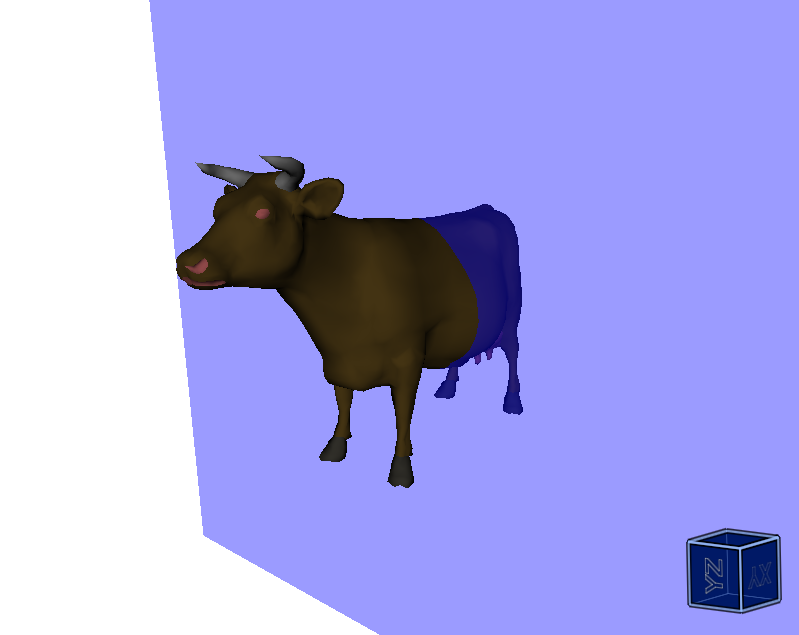
\includegraphics[width=0.3\textwidth]{ownChapters/figures/planeRotate90_010.png}%
\hspace{5.00mm}
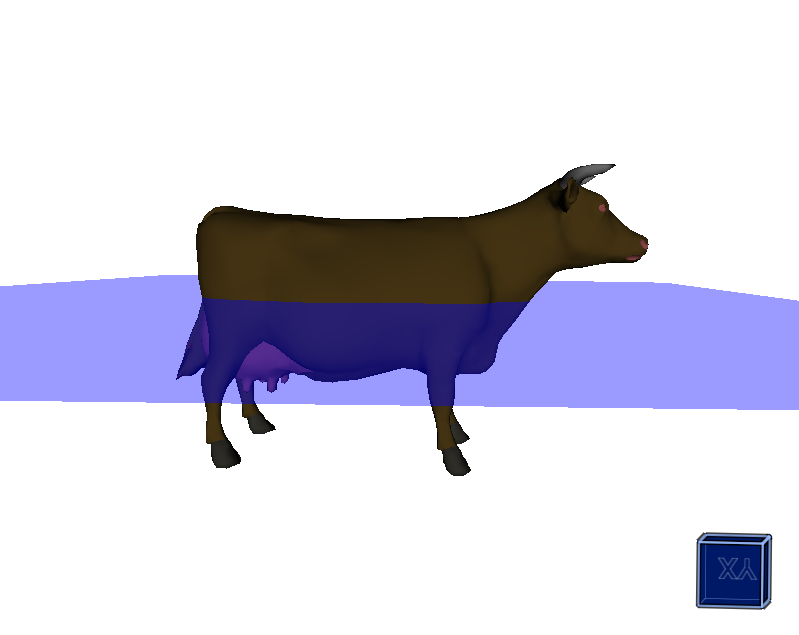
\includegraphics[width=0.3\textwidth]{ownChapters/figures/planeRotate90_100.png}%
\hspace{5.00mm}
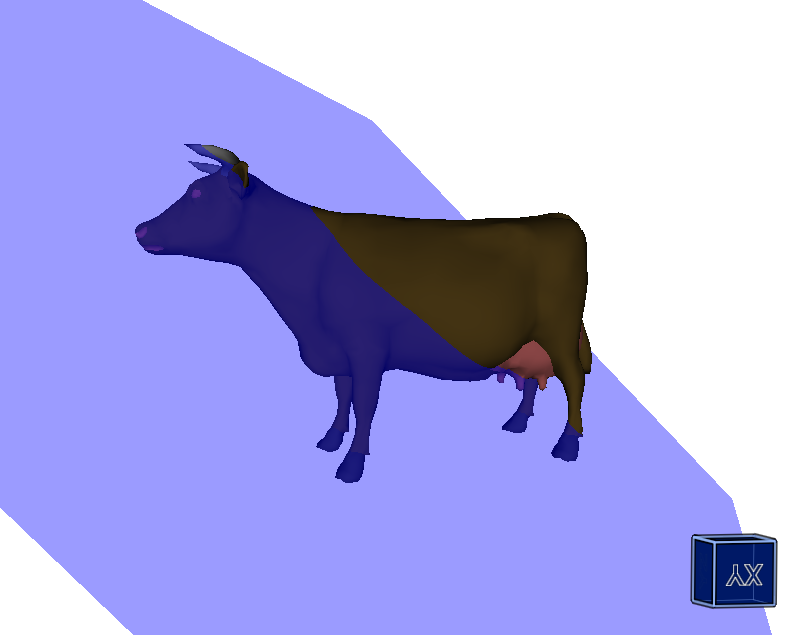
\includegraphics[width=0.3\textwidth]{ownChapters/figures/planeRotate90_101.png}%
\caption{Example of a plane with different rotation vectors. From left to right: (0,1,0), angle = 90; (1,0,0), angle = 90; (1,0,1), angle = 90}%
\label{fig:plane}%
\end{figure}

\section{Splitting the mesh}

The splitting offset is again implemented as an interface parameter. If the parameter is set to '0.0f' the mesh does not seem to be split. The larger the value of the offset the bigger the distance between the two halves of the mesh.
\begin{lstlisting}
GetPlugin().GetProperty("Offset").require(Variant::TypeFloat(0.5f));
\end{lstlisting}

Note that an observer needs to be added as well (see chapter ~\ref{chap:planeDefinition} and ~\ref{chap:observers}).

\subsection{Rotation of the planes' normal vector}
The normal of the plane has been defined as (0.0, 0.0, 1.0), but regarding that the normal vector is still located in the object space of the plane, it needs to be transformed into the same space as the mesh. This is being done by rotating the normal by the same amount as the plane is rotated in the interface.\\
The following code reveals the rotation matrix regarding the interface inputs.
\begin{lstlisting}
glLoadIdentity();
glRotatef(vecPlaneRotationAngle, vecPlaneRotationVector.GetX(), vecPlaneRotationVector.GetY(), vecPlaneRotationVector.GetZ());
\end{lstlisting}
Of course, the rotation matrix could also be calculated using the generally known formulas~\cite{book:computerGraphicsHill}:\\ %p217
\newline
x-roll:
\begin{equation}
R_{x}(\beta) = 
\begin{pmatrix} 
	1 & 0 & 0 & 0 \\ 
	0 & \cos(\beta) & -\sin(\beta) & 0 \\ 
	0 & \sin(\beta) & \cos(\beta) & 0 \\ 
	0 & 0 & 0 & 1 
\end{pmatrix}
\end{equation}
\newline
y-roll:\\
\begin{equation}
R_{y}(\beta) =
\begin{pmatrix} 
	\cos(\beta) & 0 & \sin(\beta) & 0 \\
	0 & 1 & 0 & 0 \\
	-\sin(\beta) & 0 & \cos(\beta) & 0 \\
	0 & 0 & 0 & 1
\end{pmatrix}
\end{equation}
\newline
z-roll:\\
\begin{equation}
R_{z}(\beta) =
\begin{pmatrix} 
	\cos(\beta) & -\sin(\beta) & 0 & 0 \\
	\sin(\beta) & \cos(\beta) & 0 & 0 \\
	0 & 0 & 1 & 0 \\
	0 & 0 & 0 & 1
\end{pmatrix}
\end{equation}
\newline
% book p 220
However, it should be considered that 3D rotation matrices do not commute~\cite{book:computerGraphicsHill}, so the order of multiplication matters. For details on matrix multiplication and applying affine transformations please look up the referenced literature\cite{book:computerGraphicsHearn}\cite{book:computerGraphicsHill}.
\newline
Subsequently, the rotated normal vector is multiplied with the model view matrix to get the vector in model view space before it is normalized. After normalization the normal vector has a value between 0 and 1.
\begin{lstlisting}
planeNormal.normalize();
\end{lstlisting}

\subsection{Translating the mesh}
After the light calculations the mesh is translated by the value of the offset in the direction of the normal vector. The command in OpenGL for translation is 'glTranslatef'. Before the mesh is rendered the shader needs to be bound.
\begin{lstlisting}
Vector meshTranslation = planeNormal * offset;
glTranslatef(meshTranslation.GetX(), meshTranslation.GetY(), meshTranslation.GetZ());
m_shaShader.bind();
renderMesh(*pMesh);
m_shaShader.release();
\end{lstlisting}
As stated above the mesh is rendered twice to create the illusion of a mesh that is dragged apart. Therefore, the mesh needs to be rendered again with a translation in the opposite direction.\\
In VolumeShop, the two meshes are displayed with a plane in between. The distance of the meshes is twice the offset (see chapter~\ref{fig:offset}).

\begin{figure}%
\centering
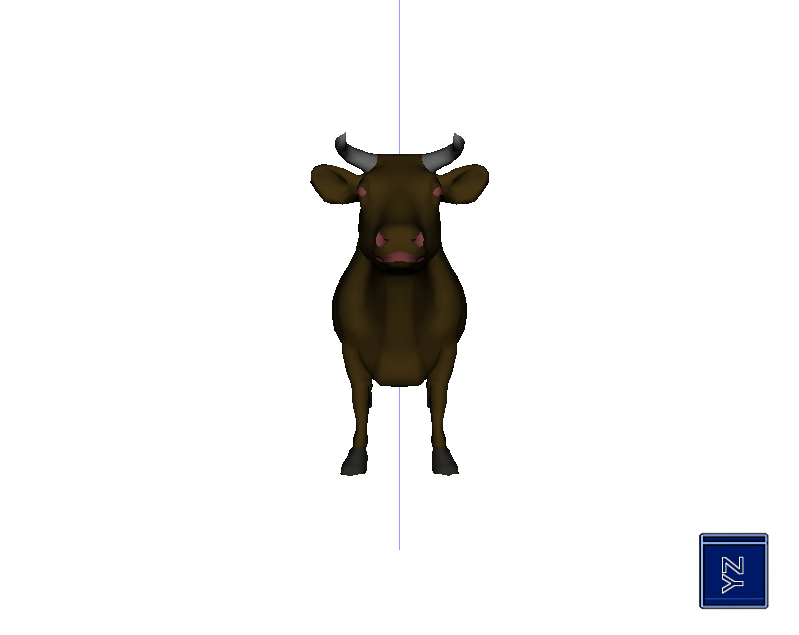
\includegraphics[width=0.4\textwidth]{ownChapters/figures/1_noOffset.png}%
\hspace{7.00mm}
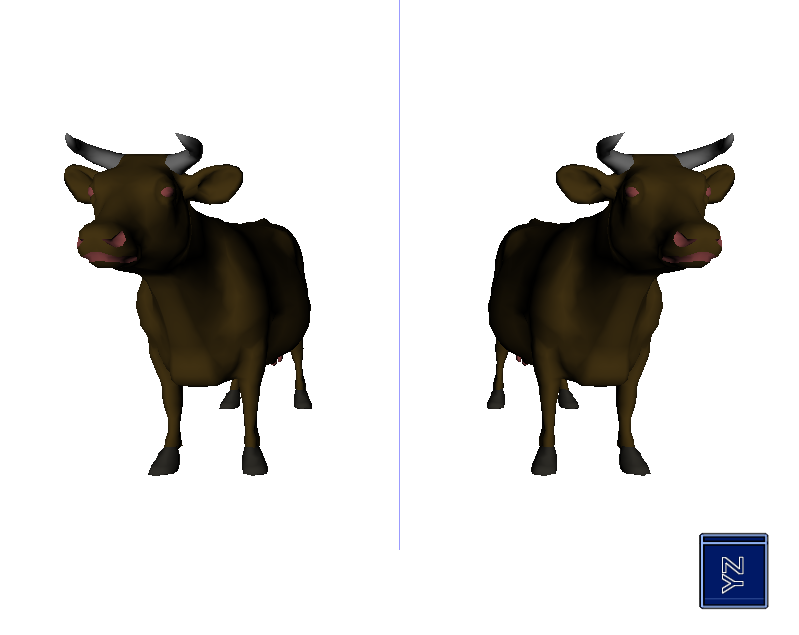
\includegraphics[width=0.4\textwidth]{ownChapters/figures/2_offset.png}%
\caption{The mesh with no offset (left) and with offset applied (right)}%
\label{fig:offset}%
\end{figure}


\subsection{Discarding dispensable fragments}
To eliminate the pixels from the other side of the plane of each mesh respectively, it has to be determined on which side of the plane a pixel lies.\\
The computation is performed in the fragment shader.\\
The dot product of the plane normal and the vertex position minus a point on the plane states if the vertex is in front of or behind the plane. If the resulting value is smaller or equal to zero, the point is behind the plane and should not be drawn. Before the mesh is rendered, the normal of the plane as well as a point on the plane must be passed to the shader as uniforms\footnote{A uniform is a type designation. It is passed from the application to the shader. Its value in the shader is constant and never changes.~\cite{misc:glslTut}}. 
For the first half of the mesh the normal vector remains unchanged, for the second one converted. The point on the plane has to be determined in respect of the plane translation.\\
\newline
Definition of the plane normal and point on the plane as uniforms:
\begin{lstlisting}
glUniform3f(m_shaShader.GetUniformLocation("planeNormal"), planeNormal.GetX(), planeNormal.GetY(), planeNormal.GetZ());
glUniform3f(m_shaShader.GetUniformLocation("planePoint"), vecPlaneTranslation.GetX(), vecPlaneTranslation.GetY(), vecPlaneTranslation.GetZ());
\end{lstlisting}

The fragment shader discards the points behind the plane:
\begin{lstlisting}
float dotProduct = dot((vertexPosition - pointOnPlane), planeNormal);
		
if(dotProduct <= 0.0) {
	discard;
}
\end{lstlisting}

\section{Shading the mesh}
The back faces of the mesh still have the same color as the front faces, what makes it look unreal (see figure ~\ref{fig:shading}). Therefore, the back faces have to be shaded in a different color. GLSL has an input variable \emph{gl\_FrontFacing} to check if the fragment is front facing. The following code shades all back facing vertices red:
\begin{lstlisting}
if(!gl_FrontFacing){
	gl_FragColor = vec4(1.0, 0.0, 0.0, 1.0)
}
\end{lstlisting}

\subsection{Shading the back facing fragments}
To add the impression of depth, lighting of the back facing fragments is being done using the Blinn-Phong shading model~\cite{book:computerGraphicsHearn}.
\begin{lstlisting}
void directionalLight(in gl_LightSourceParameters light, in vec3 N, in vec3 V, in float shininess, inout vec4 ambient, inout vec4 diffuse, inout vec4 specular)
{
	vec3 L = normalize(light.position.xyz);
	 
	float nDotL = dot(N, L);
	 
	if (nDotL > 0.0)
	{   
		vec3 H = normalize(light.halfVector.xyz);
			 
		float pf = pow(max(dot(N,H), 0.0), shininess);

		diffuse  += light.diffuse  * nDotL;
		specular += light.specular * pf;
	}
	 
	ambient  += light.ambient;
}

void main()
{
	vec3 v = normalize(vVertexPosition);
	vec3 n = normalize(vVertexNormal);
	
	if(!gl_FrontFacing) {
		directionalLight(gl_LightSource[0], -n, v, 0.7, ambient, diffuse, specular);
		color.rgb  = ((ambient  * vec4(1.0, 0.1, 0.0, 1.0)) + (diffuse  * vec4(1.0, 0.1, 0.0, 1.0)) + (specular * vec4(1.0, 1.0, 1.0, 1.0))).rgb;			
		color.a = 1.0;			
		color = clamp(color, 0.0, 1.0);
	}
	gl_FragColor = color;
}
\end{lstlisting}

The result is a nicly shaded inside of the mesh with a hollow appearence (see figure ~\ref{fig:shading}).

\subsection{Shading the cut surface}
"`Cut surfaces are interior surfaces of solid objects that are made visible by the cutaway action."'~\cite{jour:adaptiveCutaways}\\
To smoothly shade the cut surface, the normals of the visible back-faces of the mesh are replaced by the inverse normal vector of the plane. With this approach, the shading is dependent on the viewing direction, so the reflection on the cut surface changes when the model is rotated.\\
For the implementation of shading cut surfaces, the Blinn-Phong shading model is used. So the difference to the approach stated above is simply calling the lighting function with a different normal.
\begin{lstlisting}
n = vPlaneNormal;
\end{lstlisting}
The result looks like in figure ~\ref{fig:shading}. The illustration shows a slightly rotated model to point out that the light changes with the viewing perspective, so the left half appears less illuminated than the right half.

\begin{figure}%
\centering
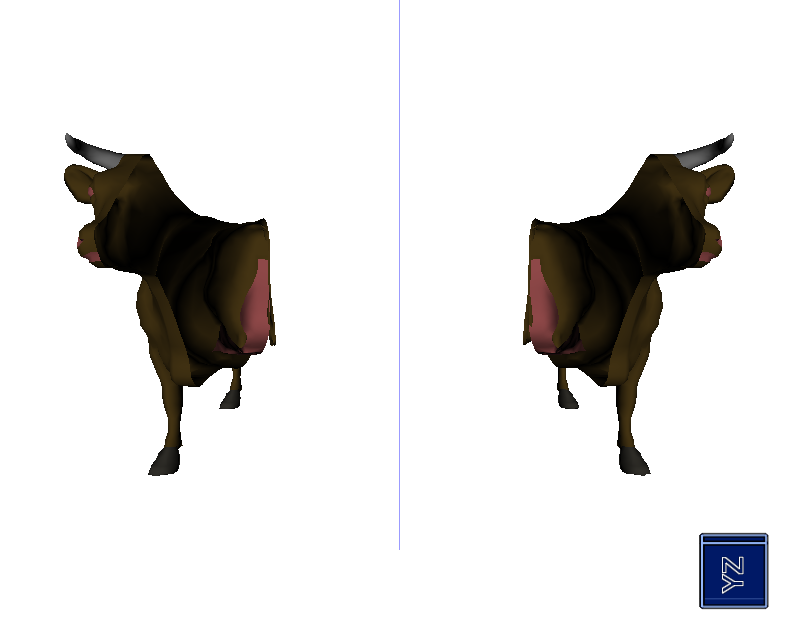
\includegraphics[width=0.4\textwidth]{ownChapters/figures/3_offset_noInside.png}%
\hspace{7.00mm}
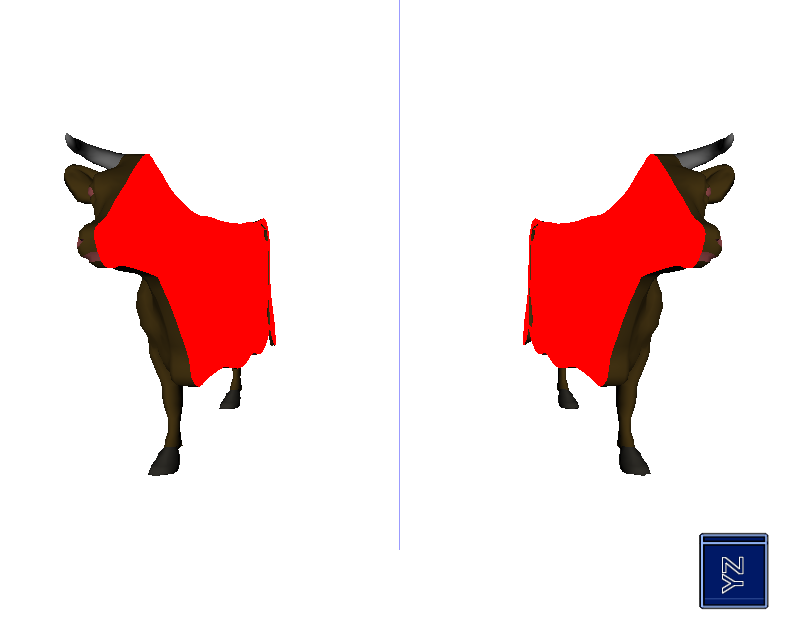
\includegraphics[width=0.4\textwidth]{ownChapters/figures/4_offset_flatInside.png}%
\hspace{7.00mm}
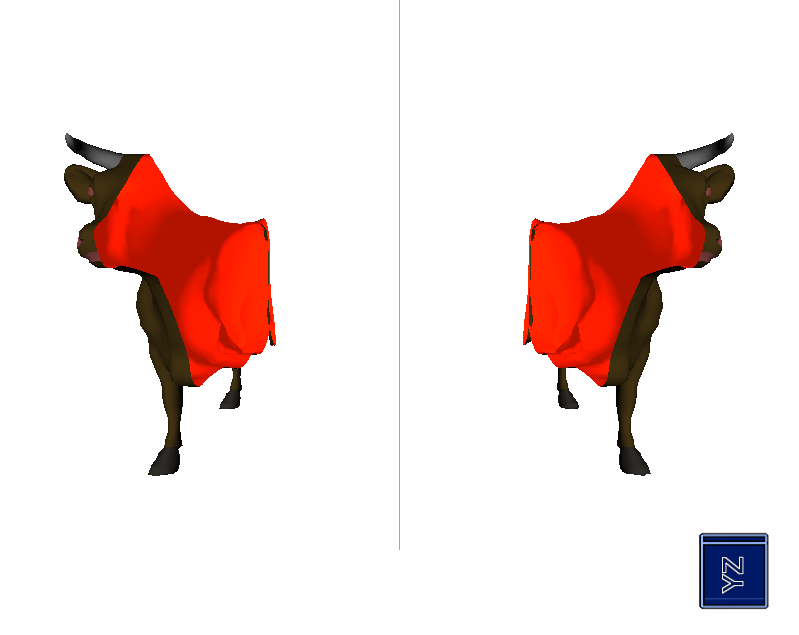
\includegraphics[width=0.4\textwidth]{ownChapters/figures/5_offset_phongInside.png}%
\hspace{7.00mm}
\includegraphics[width=0.4\textwidth]{ownChapters/figures/6_offset_paddedPhong.png}%
\caption{Different methods of shading the back faces (from upper left to lower right): no special treatment, flat shading, caved interior shading, cut surface shading}%
\label{fig:shading}%
\end{figure}
